%\addcontentsline{toc}{chapter}{Development Process}
\chapter{Design}

Once an idea of which technologies to use in the software became prevalent, a design and structure of the application had to be created, based upon the requirements and user stories outlined in Appendix A, section~\ref{user_stories}. This involves a 'big picture' overview of each component of the application, where it is judged as to how to split the components. Later on in the design stages, planning, including through the use of entity-relationship modelling, and class diagrams for object-oriented components, was carried out on each specific component of the software.

This chapter will discuss the design choices made, and link them to the software's requirements. It will include any diagrams that were completed as part of this.
\newpage
\section{Overview}

\subsection{Architecture}
\begin{figure}[!ht]
	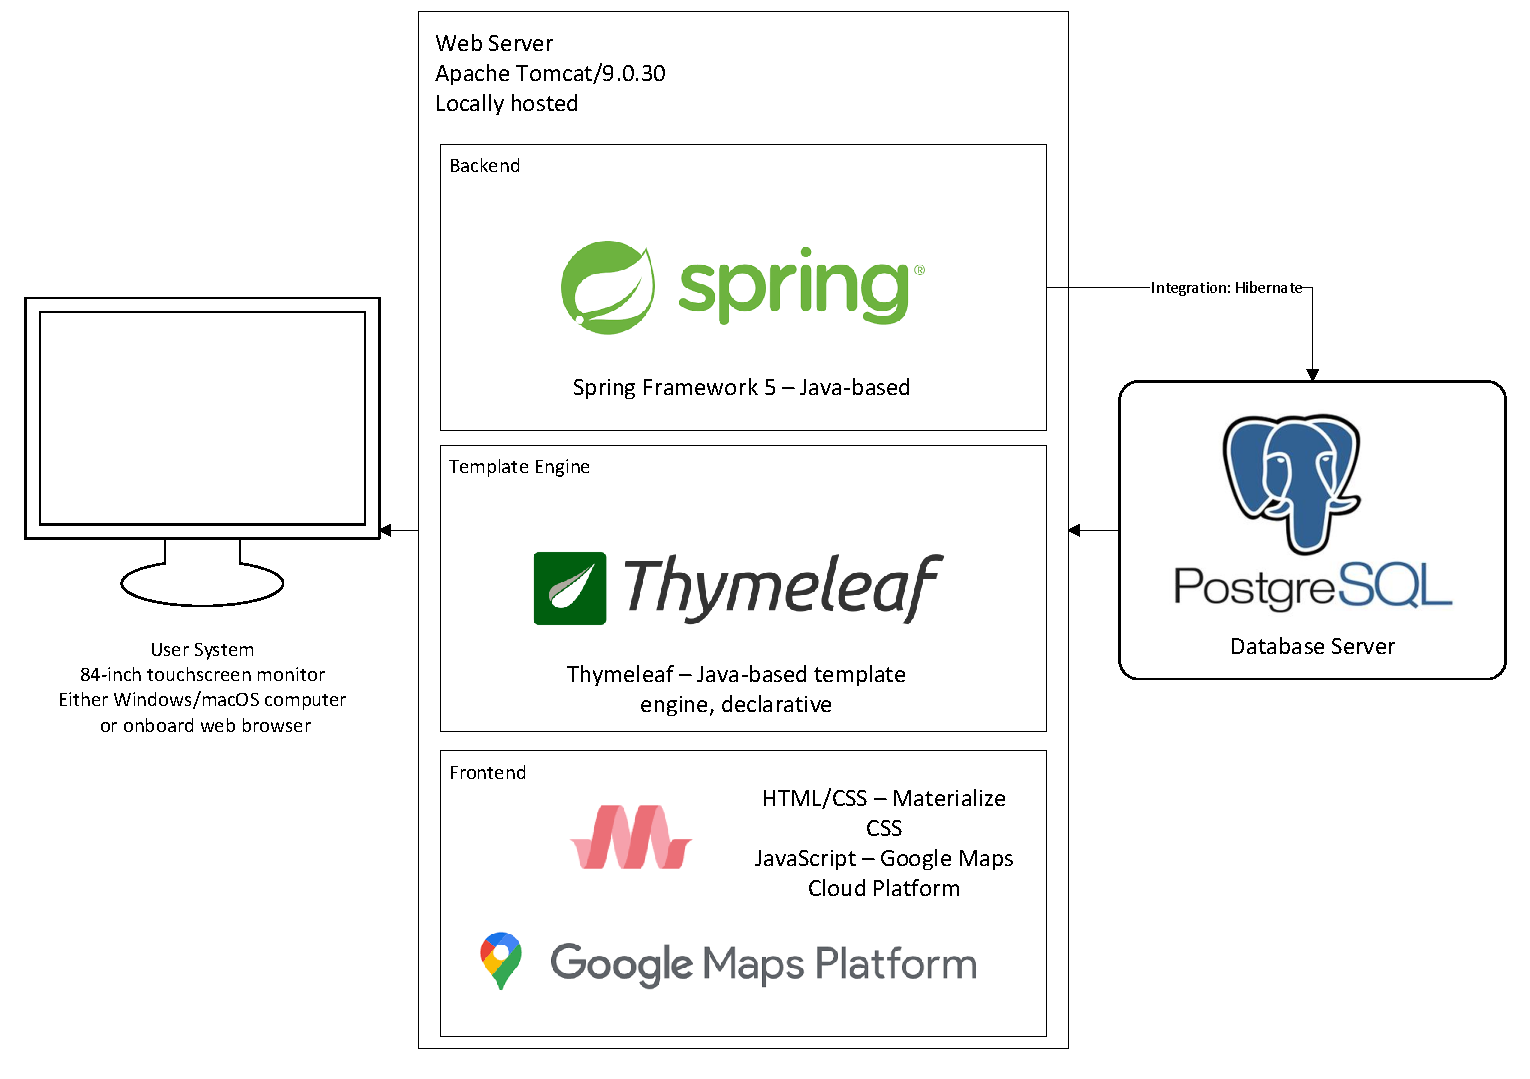
\includegraphics[scale=0.5]{diagrams/architecture_diagram}
	\caption{Architecture diagram for the Dyfi Wildlife Centre Web App}
\end{figure}	

Developing an architecture diagram ensured that there was a definition to the technology stack that the application is going to use. It also allowed for some prior thought to how different components interact with eachother.

For example, the database management system being used is PostgreSQL. Unlike systems such as SQLite, which is generally provided as a standalone file, PostgreSQL requires its own server instance. Therefore, research had to take place as to how the backend, running on Spring, would interface with the SQL Server. As evidenced in Figure 2.1, this was through Hibernate, an implementation of the standard Java persistence API for Spring's enterprise-level dialect. This was marked as something to research when planning the design for the model and controller layers of the backend.

The architecture diagram also identifies the relationships between each component hosted on the web server, in a downwards fashion. The Spring Framework interfaces with Thymeleaf, through Spring passing parameters to Thymeleaf templates, for them to be rendered. The frontend and User Experience components of the application are clearly defined - with Materialize being used for the CSS layout, and the Google Maps Cloud Platform's JavaScript API being used for displaying the map and its markers. On the left-hand side, the user's system is explicitly mentioned, as User Experience is an important consideration in this project. The user will also be interacting directly with the system and its various components that are locally hosted on the web server.

\section{Database}

Parts of the database model were able to be generated automatically using the Spring Data JPA, however it was decided that a pre-built implementation of the database model would be easier to implement, as this would ensure adherence to an entity-relationship diagram, as well as any constraints that had been identified.

The initial iteration of the database, to fulfil the first two tasks that had been defined, was to have a single relation containing details about a Point of Interest. It was decided to initially plan the database in un-normalised form. This was to ensure that the Java object that was to be created in the back-end was readable and easy to maintain, rather than having to create multiple Java objects that represent a large number of relations in the database.

The database was to be iterated upon. To allow for authentication, separate tables for users and roles were to be created. While the consideration with regards to authentication was that every user should be automatically granted admin permissions, the role database allows for further addition of new roles, should this become a concern in a later version of the project.

\subsection{Entity-Relationship Modelling}
\begin{figure}[!ht]
	\caption{Second iteration of the Dyfi Wildlife Centre schema}
	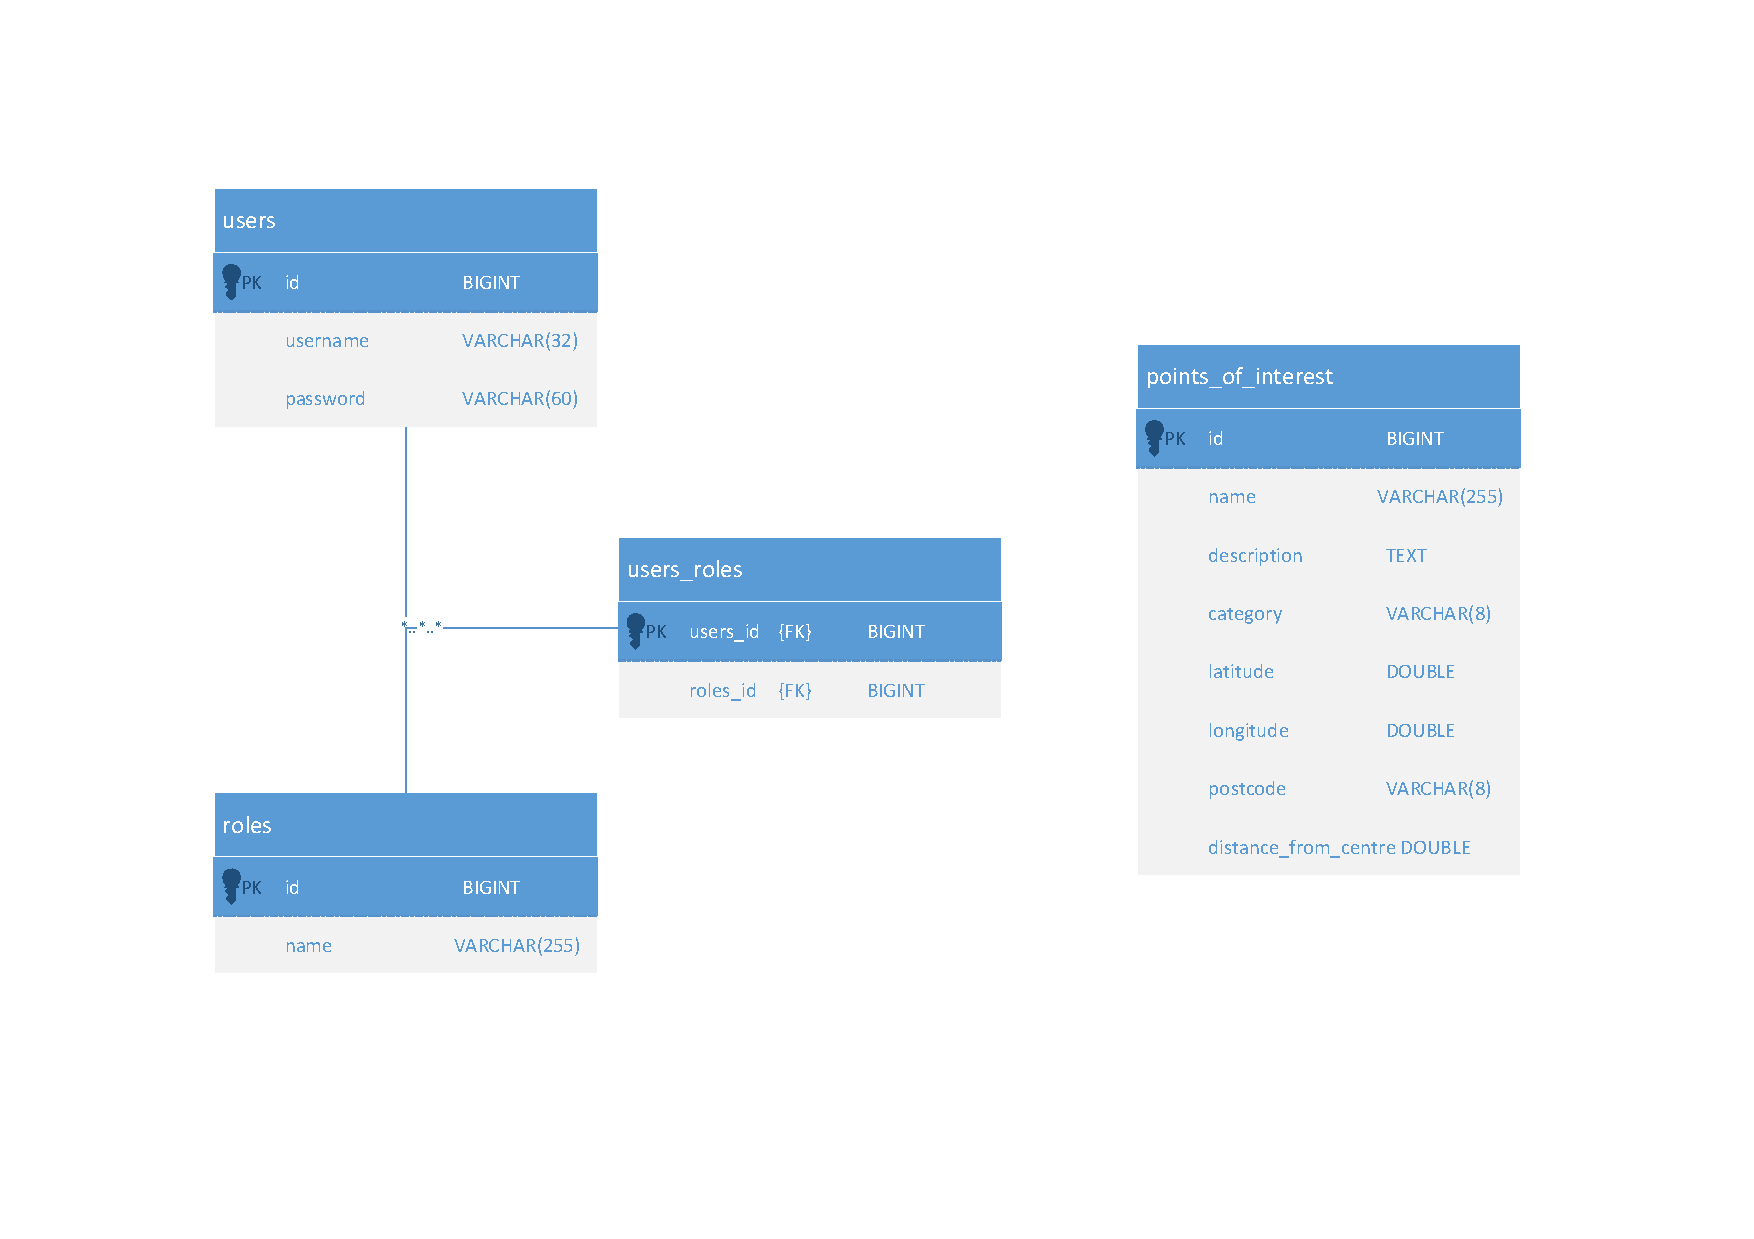
\includegraphics[scale=0.5]{diagrams/er_diagram}
\end{figure}	

Ultimately, the database design was uncomplicated, as there were only three objects to consider. As the majority of database handling was intended to be carried out through the Spring Data JPA, the nuances that that brings were added into the database at time of design. One example would be the ID primary key on each relation. In a standard PostgreSQL database implementation, the data type of the ID is not likely to be of type \textit{bigint}. This is a type that is, as the name implies, intended for large integers. An ID attribute that is being utilised as a primary key would generally take the type of \textit{serial} - an auto-incrementing column. This is, however, handled within the backend by the JPA, through an automatically-generated sequence stored within the database, therefore there is no need to use the serial type.

It is also true that, in a standard database, there would be an argument for not having an automatically-generated primary key, and instead using another unique property, such as name, or a compound primary key. However, this implementation was chosen as it allowed for faster efficiency within the backend layer of the application - a primitive type would be able to be matched faster than a String object with a string-matching algorithm behind it.

A many-to-many relationship between both users and roles is achieved through the use of a junction able, \textit{users\_roles}. This allows for multiple roles to be added into the database at a later date, which can then be attributed to users through the frontend. As each user is only permitted to have one role, the primary key has been set as the user in the junction table, with a role ID being set with each user.

\subsection{Constraints}

Constraints had to be created in order to validate the data that was being entered into the table, this is described below, with the definition in a pseudo-code format:

% Please add the following required packages to your document preamble:
% \usepackage{graphicx}
\begin{table}[h]
\centering
\resizebox{\textwidth}{!}{%
\begin{tabular}{|l|l|}
\hline
\textbf{Constraint Name}                   & \textbf{Definition}                                    \\ \hline
\textbf{latitude\_chk}                     & CHECK latitude IS \textgreater -90 AND \textless 90    \\ \hline
\textbf{longitude\_chk}                    & CHECK longitude IS \textgreater -180 AND \textless 180 \\ \hline
\textbf{latitude\_not\_null\_island\_chk}  & CHECK latitude NOT EQUAL TO 0                        \\ \hline
\textbf{longitude\_not\_null\_island\_chk} & CHECK longitude NOT EQUAL TO 0                        \\ \hline
\textbf{chk\_name}                         & CHECK name IS NOT EMPTY                                \\ \hline
\textbf{postcode\_chk}                     & CHECK postcode MATCHES UK postcode regex               \\ \hline
\end{tabular}%
}
\caption{A list of constraints in the points\_of\_interest relation}
\label{poi_constraints}
\end{table}

These constraints tend to perform sanity checks on the input that is being entered, once it reaches the database layer. The constraints on the coordinates are based upon the natural constraints based upon latitude and longitude, and ensures that a user cannot apply an incorrect coordinate to a point of interest, that would likely cause an error at the frontend layer of the application.

The two ``not null island" checks make sure that a user cannot simply enter 0 as the latitude and 0 as the longitude, as this could potentially cause issues when parsing the postcode in the backend layer. The primary issue with a check like this would be that 0,0 is a valid coordinate pair. However, the customer has specified that points of interest would primarily be in the United Kingdom, which is far from this coordinate range. It is not likely that any potential coordinate pairs entered for points of interest outside the UK would be equal to these coordinates.

A regular expression, sought from an open data source that provides APIs dealing with UK postcodes\cite{PostcodeRegex}, was, again, a sanity check. It performs basic error-checking that checks the general shape of the postcode; checking it has a letter at the beginning and ends in a letter, for example. Whilst stricter regular expressions were available, these were often rather complex expressions that were computationally intensive, and still did not cover every edge case, often making their implementation futile. The design accounts for error-checking of postcodes through the use of the aforementioned API, which is further explained in section~\ref{sec:backend}. 


\section{Backend}
\label{sec:backend}

\begin{figure}[!ht]
	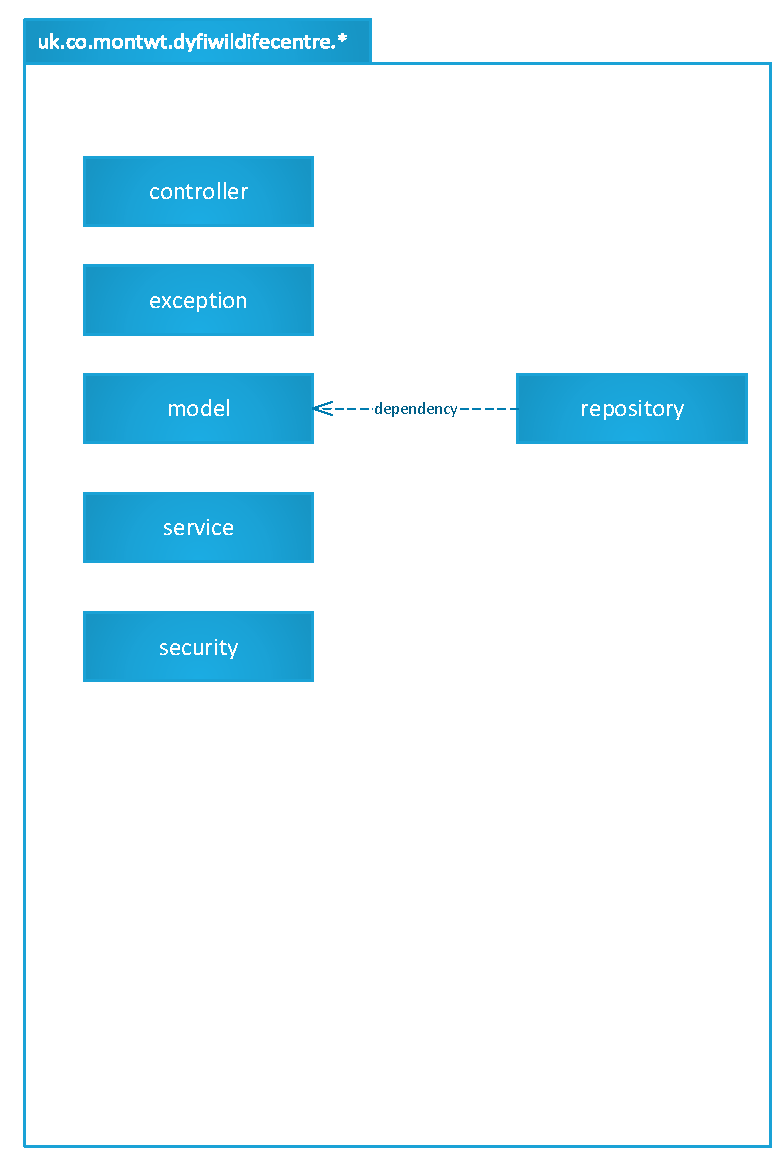
\includegraphics[scale=0.5]{diagrams/parent_uml}
	\caption{Parent UML diagram, showing each package that the software breaks down into}
\end{figure}	

Spring, the framework that is utilised in this backend, follows a model-view-controller design pattern. This allows for a clear distinction between each area of the application, with its functionalities and design being defined as follows:

\begin{itemize}
	\item	\textbf{Model} - The application's data structure and logic processing, containing the objects representing a user, a role, and a point of interest. It also includes a repository layer, that interfaces with the PostgreSQL server, and a service layer, that provides a layer of abstraction between the database and the controller.
	\item	\textbf{View} - The presentation of data in the application. This is generally further discussed in Section~\ref{sec:frontend}.
	\item	\textbf{Controller} - Classes that accept user and computer input, converting it to commands that affect either the model or the view. In this application, the controller consists of a RESTful API for managing users and points of interest.
\end{itemize}

Class diagrams were created to be adhered to during the production of this application, and were split by layer. For the sake of clarity; constructor, setter, and getter methods are not represented on the class diagram. The intention was for Java packages to be used, to aid in code navigability and ease of maintenance.

\subsection{Model layer}
\begin{figure}[!ht]
	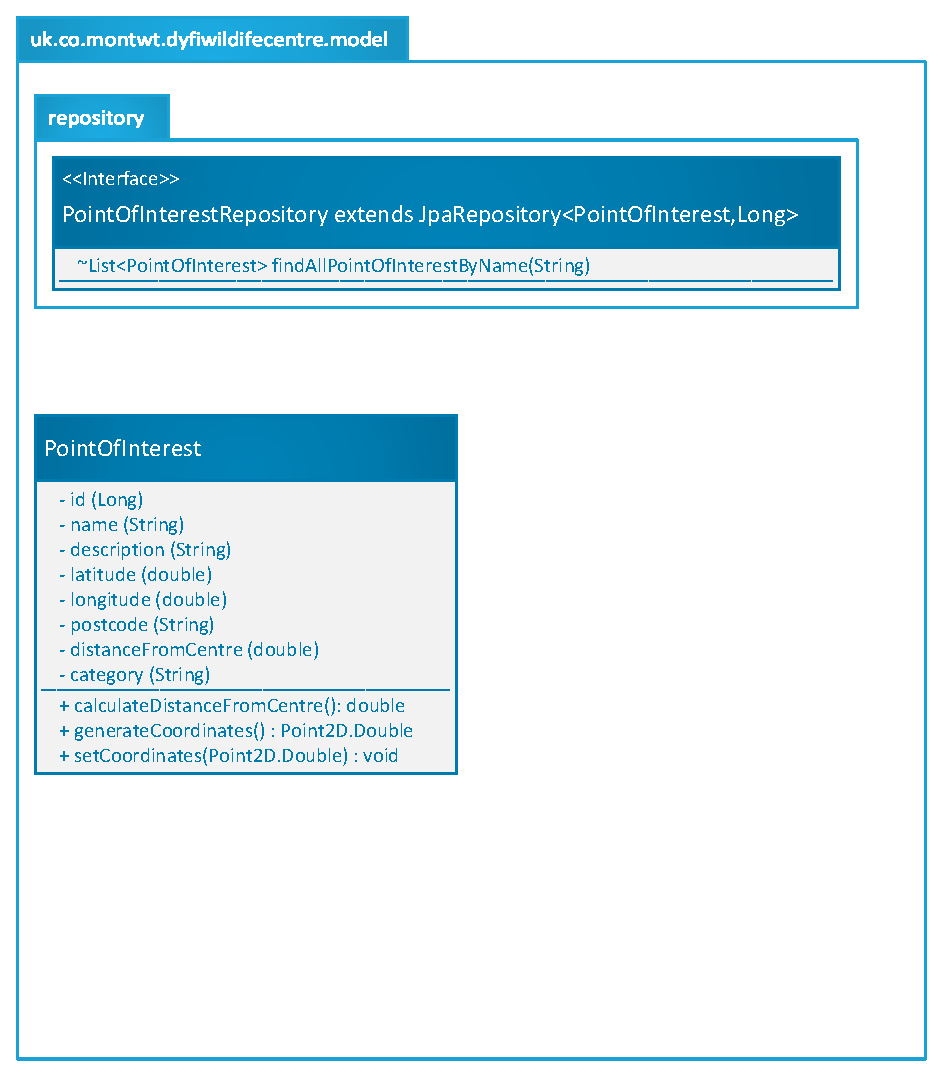
\includegraphics[scale=0.5]{diagrams/model}
	\caption{Class diagram of the \texttt{uk.co.montwt.dyfiwildlifecentre.model} package}
\end{figure}	

The primary model layer contains one class, as well as a sub-package. The sub-package contains an interface that accesses the \textit{point\_of\_interest} relation in the database, utilising a Spring Data JPA superclass. It contains one method, that is intended to invoke an SQL command directly that finds a point of interest by its name, rather than its ID.

The \texttt{PointOfInterest.java} class defines a point of interest in an identical fashion to that of the database layer. This is required by the Spring Data JPA, and results in fewer manual configurations to be carried out. It was noted that a refactoring of this class diagram could include a further class, named Location, that includes the location-based members of PointOfInterest. This could be represented in the database by a one-to-one relationship. However, at least initially, this was not to be represented in the data modelling, and as the project is being developed in an agile fashion could be refactored in the future if considered necessary.

The \texttt{calculateDistanceFromCentre()} is designed such that it calculates the great-circle distance between two pairs of coordinates, with one being the coordinates for the Dyfi Wildlife Centre. This calculation would be in miles, to four significant figures, and would help in presenting users the distance between points of interest and the visitor centre. The \textit{Haversine formula}, a formula in spherical trigonometry to determine distance between two points on a sphere, was to be implemented, with the code that was used available in Appendix C, section~\ref{haversine}.

\subsection{Controller Layer}

The controller layer at this level of the application is intended to act as a RESTful API that interfaces with a point of interest and its database. Therefore, the HTTP requests that surround the API are intended to be as clear as possible as to their intention with as much avoidance of side-effects as possible. The controller layer also includes a sub-layer, to interface between itself and the database.

\subsubsection{Services}
\begin{figure}[!htbp]
	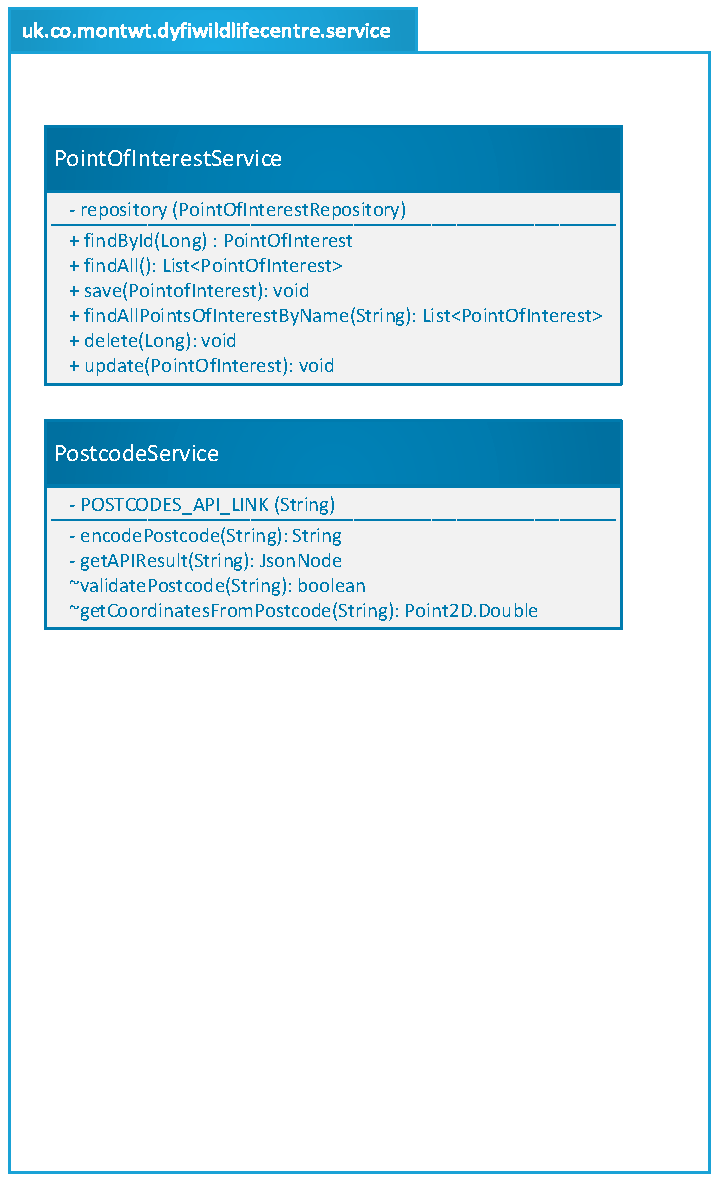
\includegraphics[scale=0.4]{diagrams/modelservice}
	\caption{Class diagram of the \texttt{uk.co.montwt.dyfiwildlifecentre.service} package}
\end{figure}	

The controller layer of this application utilises a service layer - providing an extra layer of abstraction between the database and the controller. It also includes any logic required within the methods, for example, any backend-level error-checking before the object is passed to the database.

The \texttt{PointOfInterestService.java} class manages the data transferring between the controller layer, the model layer, and the database. Method such as \texttt{findAll()} and \texttt{delete(Long id)} simply make a method call to an identical repository method, that manages the SQL transaction. However, some other methods are slightly more complicated, the most prominent example being the \texttt{save(PointOfInterest poi)} method. The method first determines if a postcode or a coordinate pair was entered into the form. If a postcode was entered, then a method call must be made to fetch the coordinates corresponding to that postcode. If not, there is no need to, however an error will occur if both a postcode and coordinates had been entered. The distance from the centre is also calculated and set in the object, before it being passed to the database.

The second service, \texttt{PostcodeService.java} manages parsing of postcodes, and includes methods to both validate a postcode, and get the coordinates that correspond to a postcode. This utilises the `postcodes.io` API, an open-source, RESTful API that utilises open data primarily provided by the Ordnance Survey, the United Kingdom's national mapping agency\cite{PostcodesAPI}. Methods in this service are used to validate a postcode - ensuring that it is a real postcode and there is information available for it, as well as looking up a postcode and extracting the given latitude and longitude. This will not be an exact location, particularly if the user is marking a place on a residential street, for example. However, coordinates can still be added manually if more precision is required, and a postcode will still provide visitors an idea of where the point of interest is. Other APIs, such as the geocoding API included in Google Maps Platform, were considered, however further analysis of the pricing model saw that there was a risk of utilisation of such an API being costly.

\subsubsection{Controllers}
\begin{figure}[!htbp]
	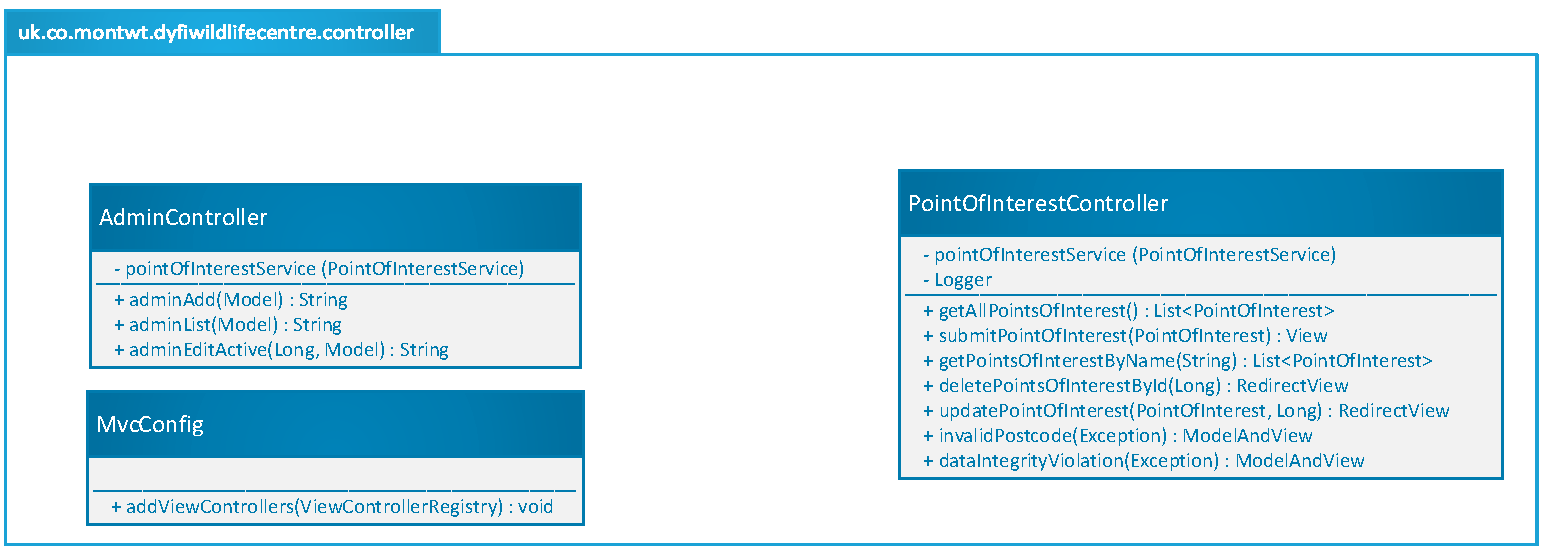
\includegraphics[scale=0.4]{diagrams/controller}
	\caption{Class diagram of the \texttt{uk.co.montwt.dyfiwildlifecentre.controller} package}
\end{figure}	

There are three controllers within this layer of the application, each with three distinct responsibilities.

The \texttt{MvcConfig.java} package is designed such as to reduce the number of methods required for simple loading of a view, with other methods designed to either include a payload in its model or related directly to the API that the controller is implementing. The class has only one method, that declaratively adds a view controller with a URL path, along with the correct view name.

\texttt{AdminController.java} controls data that is being passed to the admin panel view models, with the methods within the controller either carrying objects within its model, or having a model passed to it via a query string that is appended to the URL. Continuing with the abstraction granted through the service layer, the methods are short, simply adding attributes to the model for them to be handled in the view.

\texttt{PointOfInterestController.java} has a greater number of methods, that handle requests as a RESTful API. A brief specification is included in the table below.

% Please add the following required packages to your document preamble:
% \usepackage{graphicx}
\begin{table}[h]
\centering
\resizebox{\textwidth}{!}{%
\begin{tabular}{|l|l|l|}
\hline
\textbf{Endpoint}    & \textbf{Description}                                                                      & \textbf{Return Type}                         \\ \hline
/poi/get/id/:id      & Returns the point of interest where :id corresponds to the ID of the point of interest     & PointOfInterest                              \\ \hline
/poi                 & Returns all points of interest in the database                                            & List\textless{}PointOfInterest\textgreater{} \\ \hline
/poi/form\_create?poi=:poi &
  Saves a point of interest to the database where :poi corresponds to the point of interest to be saved &
  RedirectView \\ \hline
/poi/get/name/:name &
  Returns the points of interest where :name corresponds to the name of the point of interest &
  List\textless{}PointOfInterest\textgreater{} \\ \hline
/poi/delete?id=:id   & Deletes the point of interest where :id corresponds to the ID of the point of interest    & RedirectView                                 \\ \hline
/poi/update?poi=:poi & Updates a point of interest where :poi corresponds to the point of interest to be updated & RedirectView                                 \\ \hline
\end{tabular}%
}
\caption{API endpoints for /poi}
\label{tab:poi-endpoints}
\end{table}

Whilst RESTful values were adhered to as much as possible, HTML's incompatibility with request that are not GET or POST required methods such as delete to be HTTP GET request rather than HTTP DELETE. This will be further discussed in the Implementation chapter.


\subsection{Security}

Various information security considerations had to be taken into account whilst designing the application, the main one being authenticating and securing the administration panel. As the software is designed for use in a public location, an unauthenticated admin panel, where anybody who wants to could add or edit points of interest and users, was not acceptable. Therefore, a strategy for user authentication had to be put into place.

An example of a threat affecting the authentication of the application, once implemented, could be an SQL injection. A successful attack could expose user passwords and tamper with existing data stored in the database. If an attacker was able to gain access to the wireless network that the customer will be connecting the system to, they may be able to connect to the database remotely, resulting in physical limitations on access to hardware becoming futile. A suggestion could be made to the customer to secure their wireless network, perhaps having one SSID for public use and one for private use, however there is no way to enforce this in the application. With the application being hosted locally, it would be difficult to encrypt requests via HTTPS without creating a standalone server.

To combat these security concerns, Spring Security, an authentication framework designed for use with Spring, was implemented, through the contents of the security package. Users were stored in an SQL database, along with their roles. The default authentication method for users was plain-text, and users passwords could be easily found in the database. This was modified to use ``bcrypt", a password hashing function based upon the Blowfish cipher\cite{bcrypt}. bcrypt hashes the password that the user has been registered with, and then stores that hash in the password field of the relation. When a user logs in, the password that has been provided is matched against the hash, rather than the hash being decrypted, resulting in it not being reasonably possible to crack a password from the hash. 

\subsubsection{Model layer}
\begin{figure}[!htbp]
	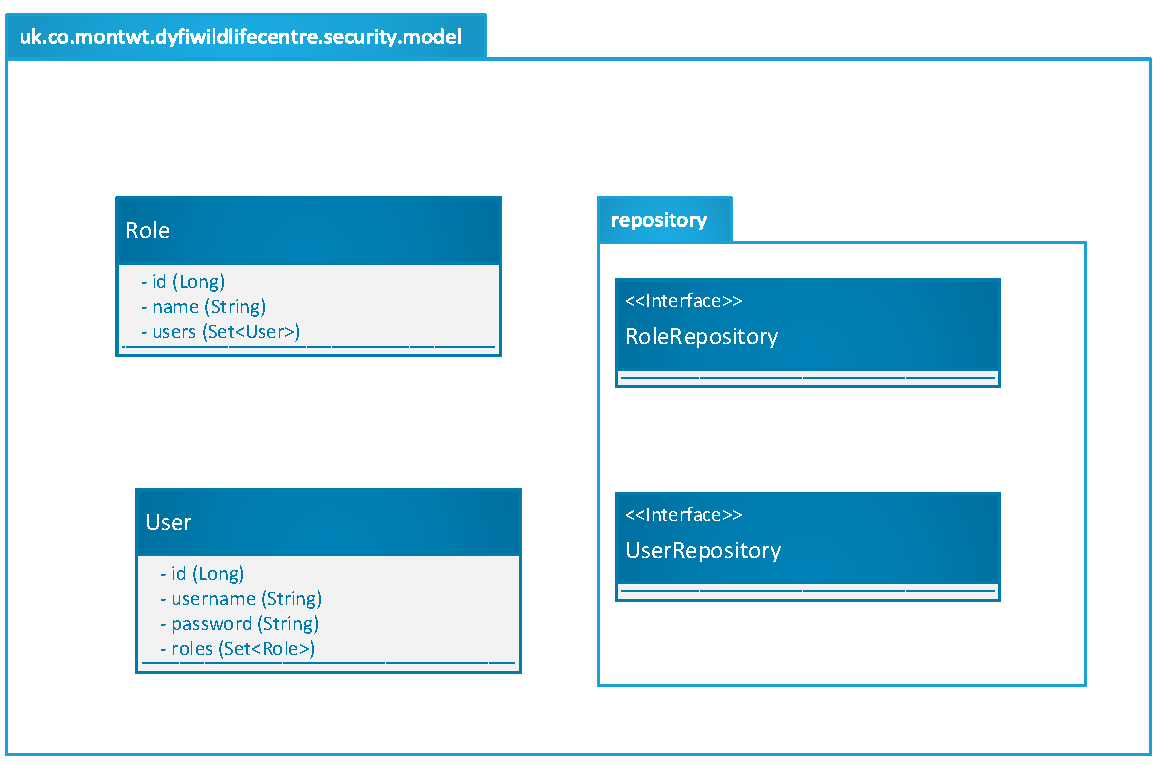
\includegraphics[scale=0.4]{diagrams/security/model}
	\caption{Class diagram of the \texttt{uk.co.montwt.dyfiwildlifecentre.security.model} package}
\end{figure}

The model layer of the security package implements the database. There are no special methods and the purpose is simply to represent the database as Java objects.

\begin{figure}[!htbp]
	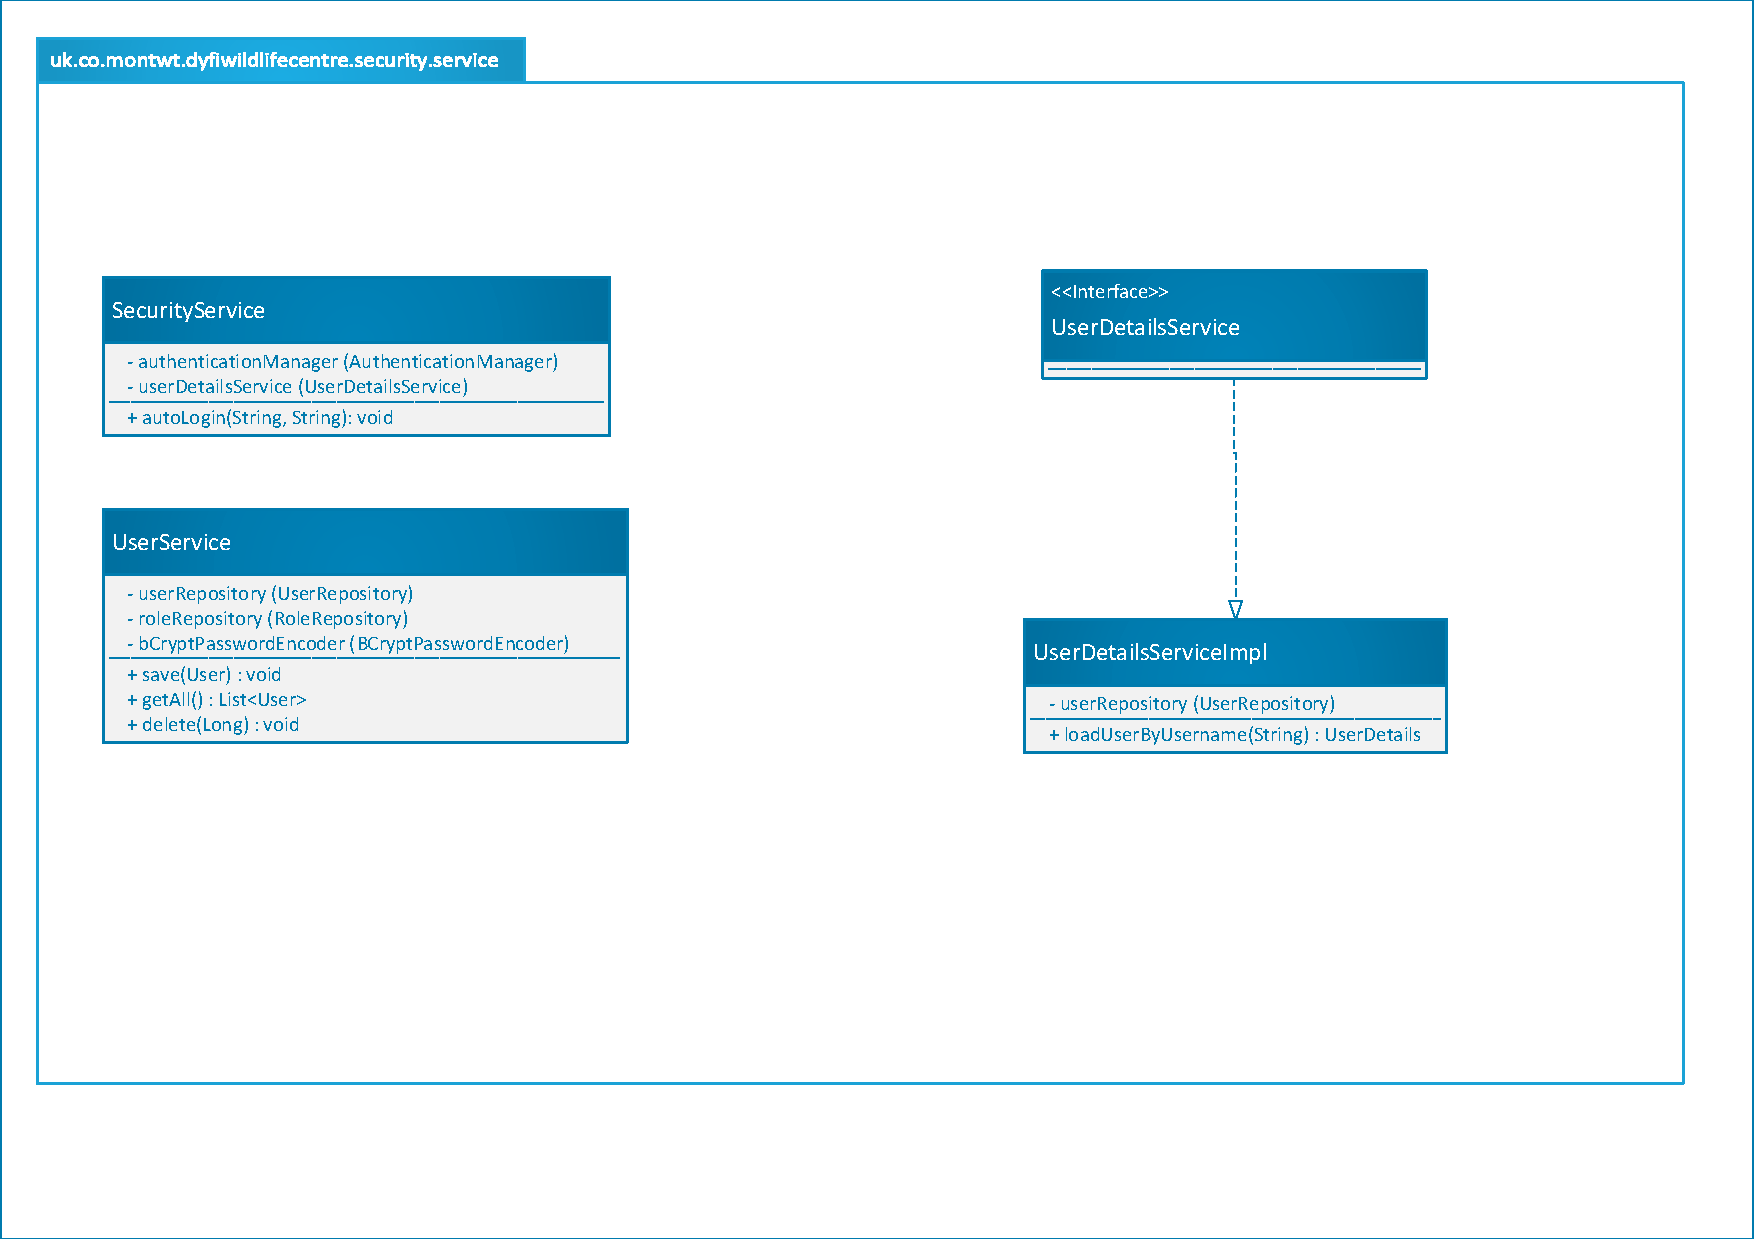
\includegraphics[scale=0.4]{diagrams/security/service}
	\caption{Class diagram of the \texttt{uk.co.montwt.dyfiwildlifecentre.security.service} package}
\end{figure}

The security layer contains implementations for an interface from the Spring Security package, as well as instantiating Spring Security's authentication manager. In the \texttt{save(User user)} method in \texttt{UserService.java}, the BCrypt encoder is called, and the password is encrypted. As discussed above, the password is sent to the service in plain text, however this would be difficult to encrypt without HTTPS, and data transfer is being carried out solely on the local host due to the nature of the locally hosted database.

\subsubsection{Controller layer}
\begin{figure}[!htbp]
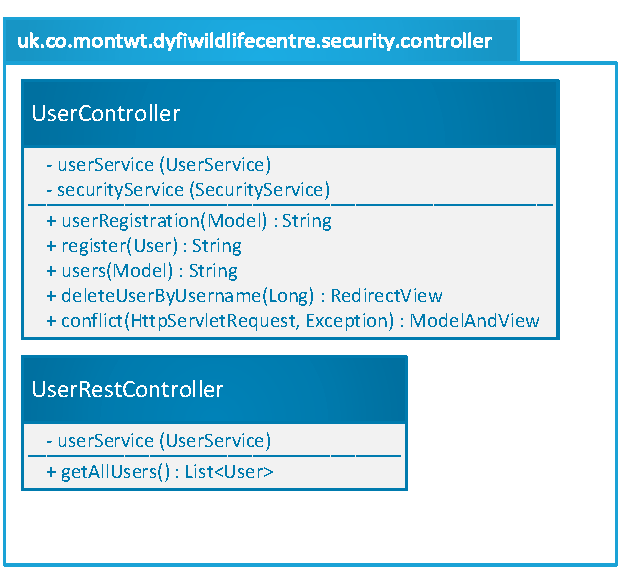
\includegraphics[scale=0.55]{diagrams/security/controller}
\caption{Class diagram of the \texttt{uk.co.montwt.dyfiwildlifecentre.security.controller} package}
\end{figure}

The controller layer of the security package includes a RESTful controller as well as a controller for the User object itself, that, as with the PointOfInterestController, interfaces with the service and the database. \texttt{UserRestController} implements a GET request, that returns all users, in order for them to be displayed in a list. \texttt{UserController} manages the registration and deletion of users, containing method calls to the relevant services. It also includes an exception handler, that reports a conflict message to the user, should they attempt to register a user with the same username as one that has already been registered.

\section{Frontend}
\label{sec:frontend}

\subsection{Design considerations}

The frontend is a crucial part of this application, as this will be what the end user will be viewing. There were some key considerations that had to take place when making decisions regarding how to design the User Experience.

Familiarity was an important consideration to make, as users may not have a large amount of technical training, and a layout that they would be used to from different applications may be beneficial. This was part of the reasoning behind choosing Material Design as the design language for this software - with most Android, and some iOS apps, using Material Design, as well as popular web services such as Google Maps, there would not be a large number of potentially confusing prompts and dialogues.

An aspect of minimalism was required with the design of the software, particularly on the homepage. The core function of the software was to show points of interest on a map, and having too many other UI components on the front page could potentially result in the page being too bloated. There was not too much of a need for a change from this in the admin panel, with clear instructions as to what the purpose of the view was.
\subsection{Prototyping}

Prototyping and mockups were created as part of the planning and design process. These mockups were based on Semantic UI, which was changed to Materialize after the mockups were created. As there were quite a few similarities, it was decided to not redesign the mockups.

\subsubsection{Home Screen}
\begin{figure}[!htbp]
\includegraphics[scale=0.2]{mockups/Home Screen}
\caption{Home Screen mockup}
\end{figure}

The initial representation of the home screen showed a menu bar, at the top of the page, along with a hamburger menu. The main component of the home screen was the Google Maps component, with filter and reset buttons on either side of it. The general shape of this mockup was carried over to the final build, however a floating action button was used in place of two distinct buttons.
\newpage
\subsubsection{Marker information}
\begin{figure}[!htbp]
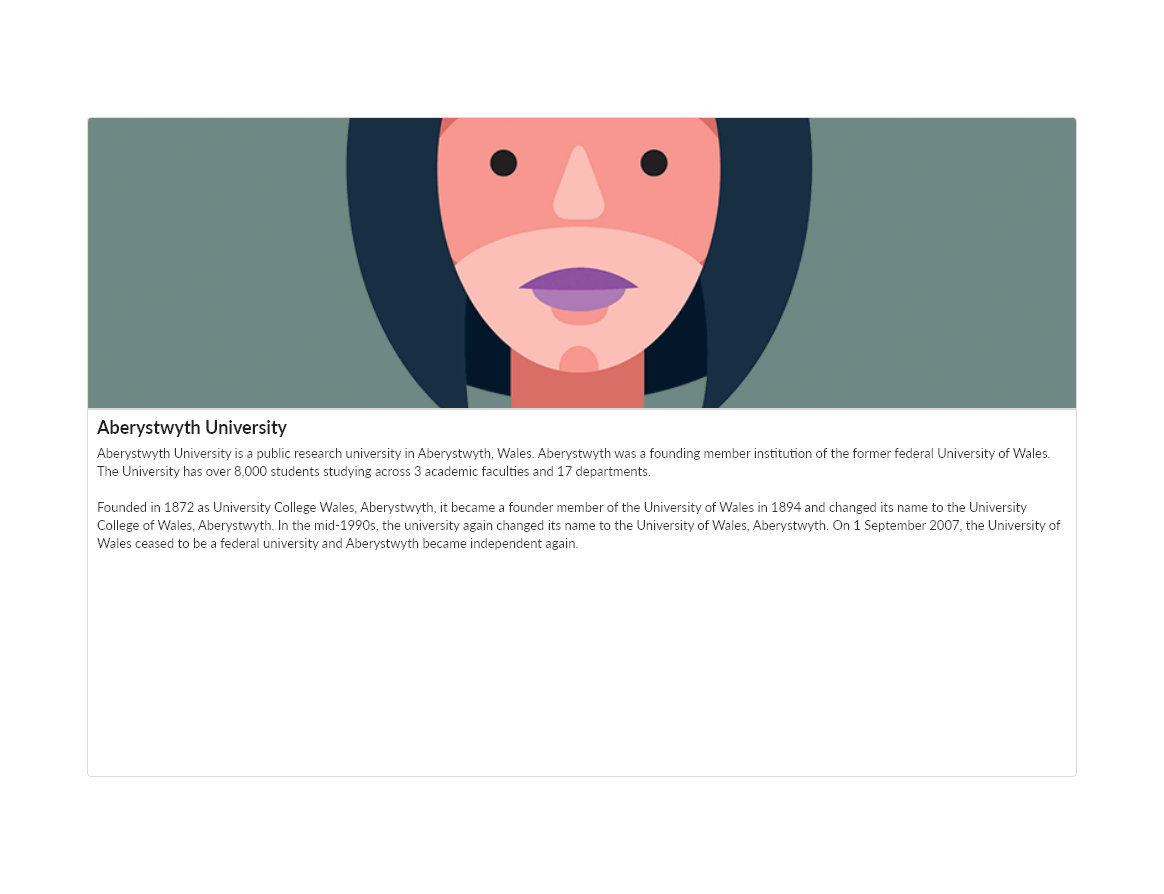
\includegraphics[scale=0.2]{mockups/POI card}
\caption{Mockup of the POI card}
\end{figure}

The `POI card` was designed such that it would contain easily-readable information, including a title, a description, and a relevant image. The POI card appears should a user click on a marker, with the JavaScript function for the Maps API being used to populate these fields. The scripts used to show the POI card are available in Appendix C.

\subsubsection{Admin Panel - Login Screen}
\begin{figure}[!htbp]
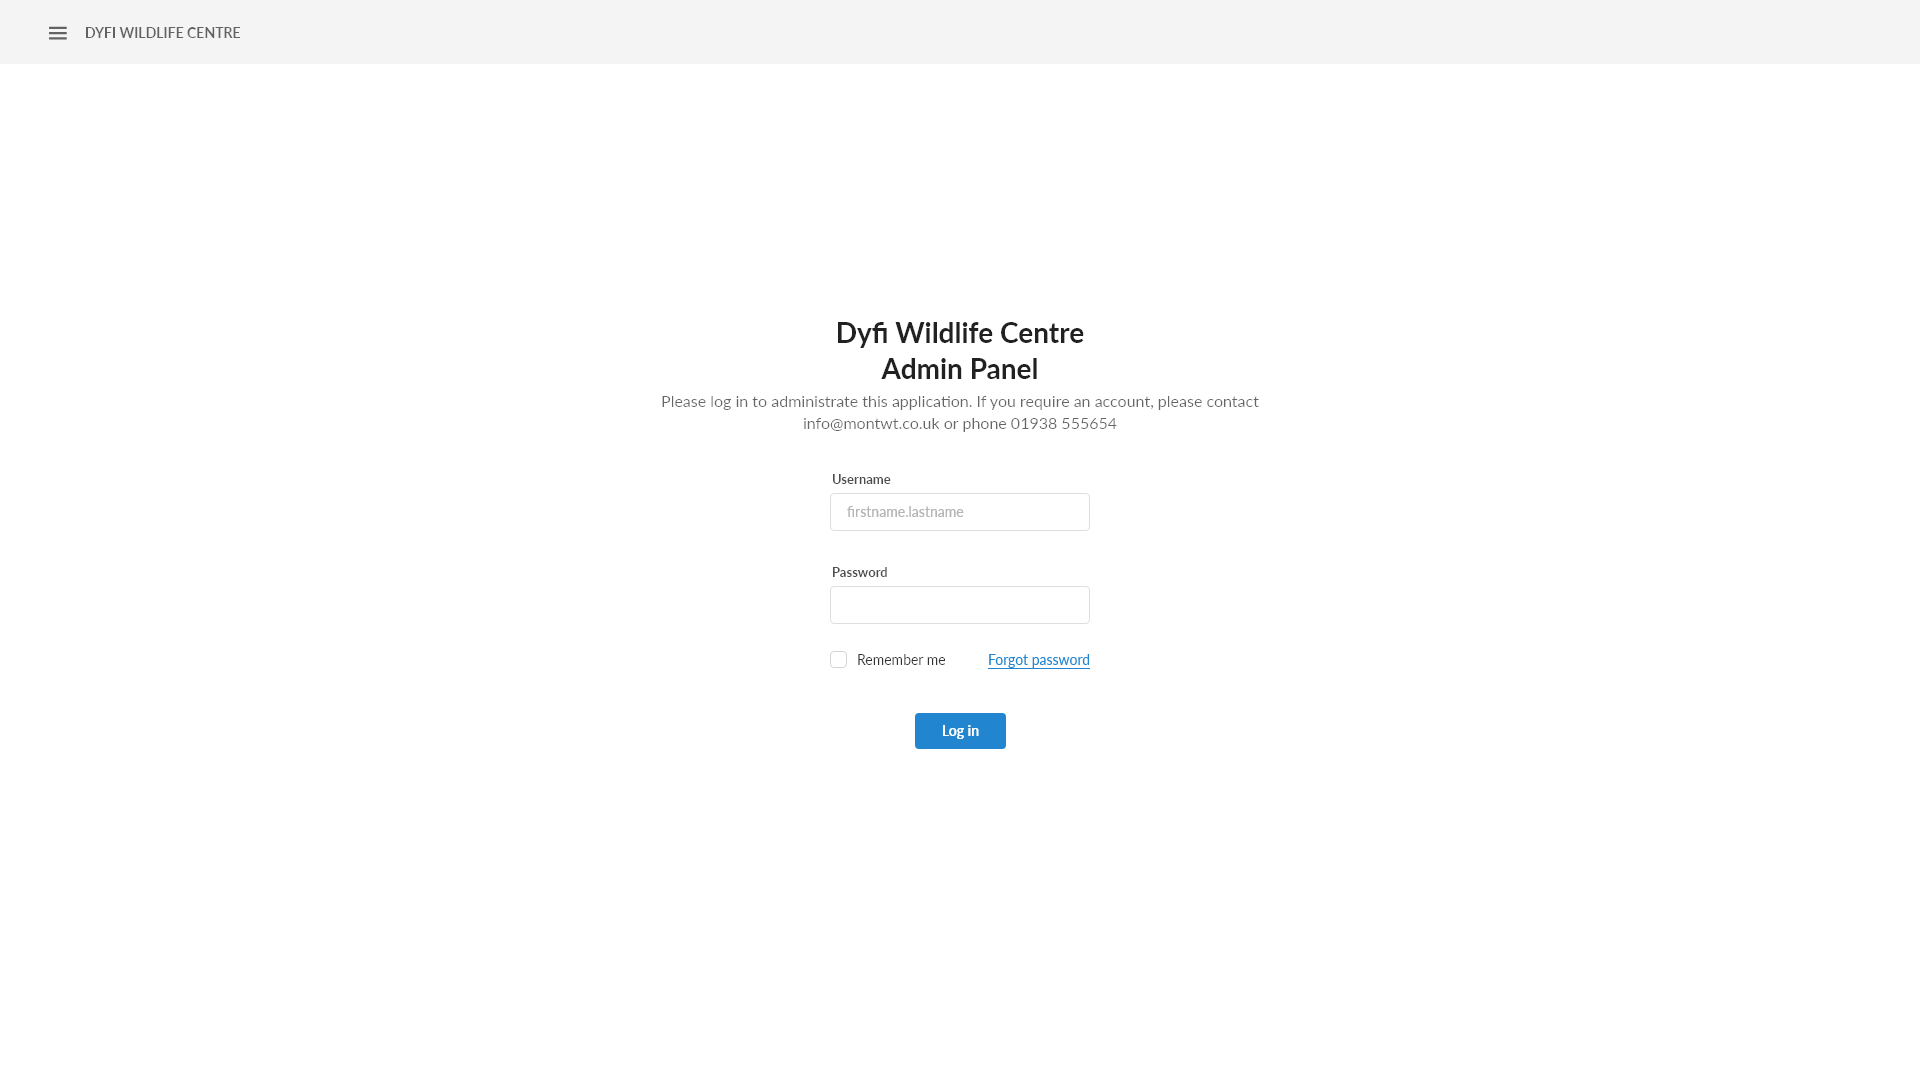
\includegraphics[scale=0.2]{mockups/Admin login screen}
\caption{Mockup of the admin login screen}
\end{figure}

As explained above, the admin login screen was designed to be as minimalistic as possible. It simply includes a username and password, as well as a brief piece of information describing how one would go about requesting a login for the admin panel. Spring Security is used to facilitate the login.

\subsubsection{Admin Panel - POI editing}
\begin{figure}[!htbp]
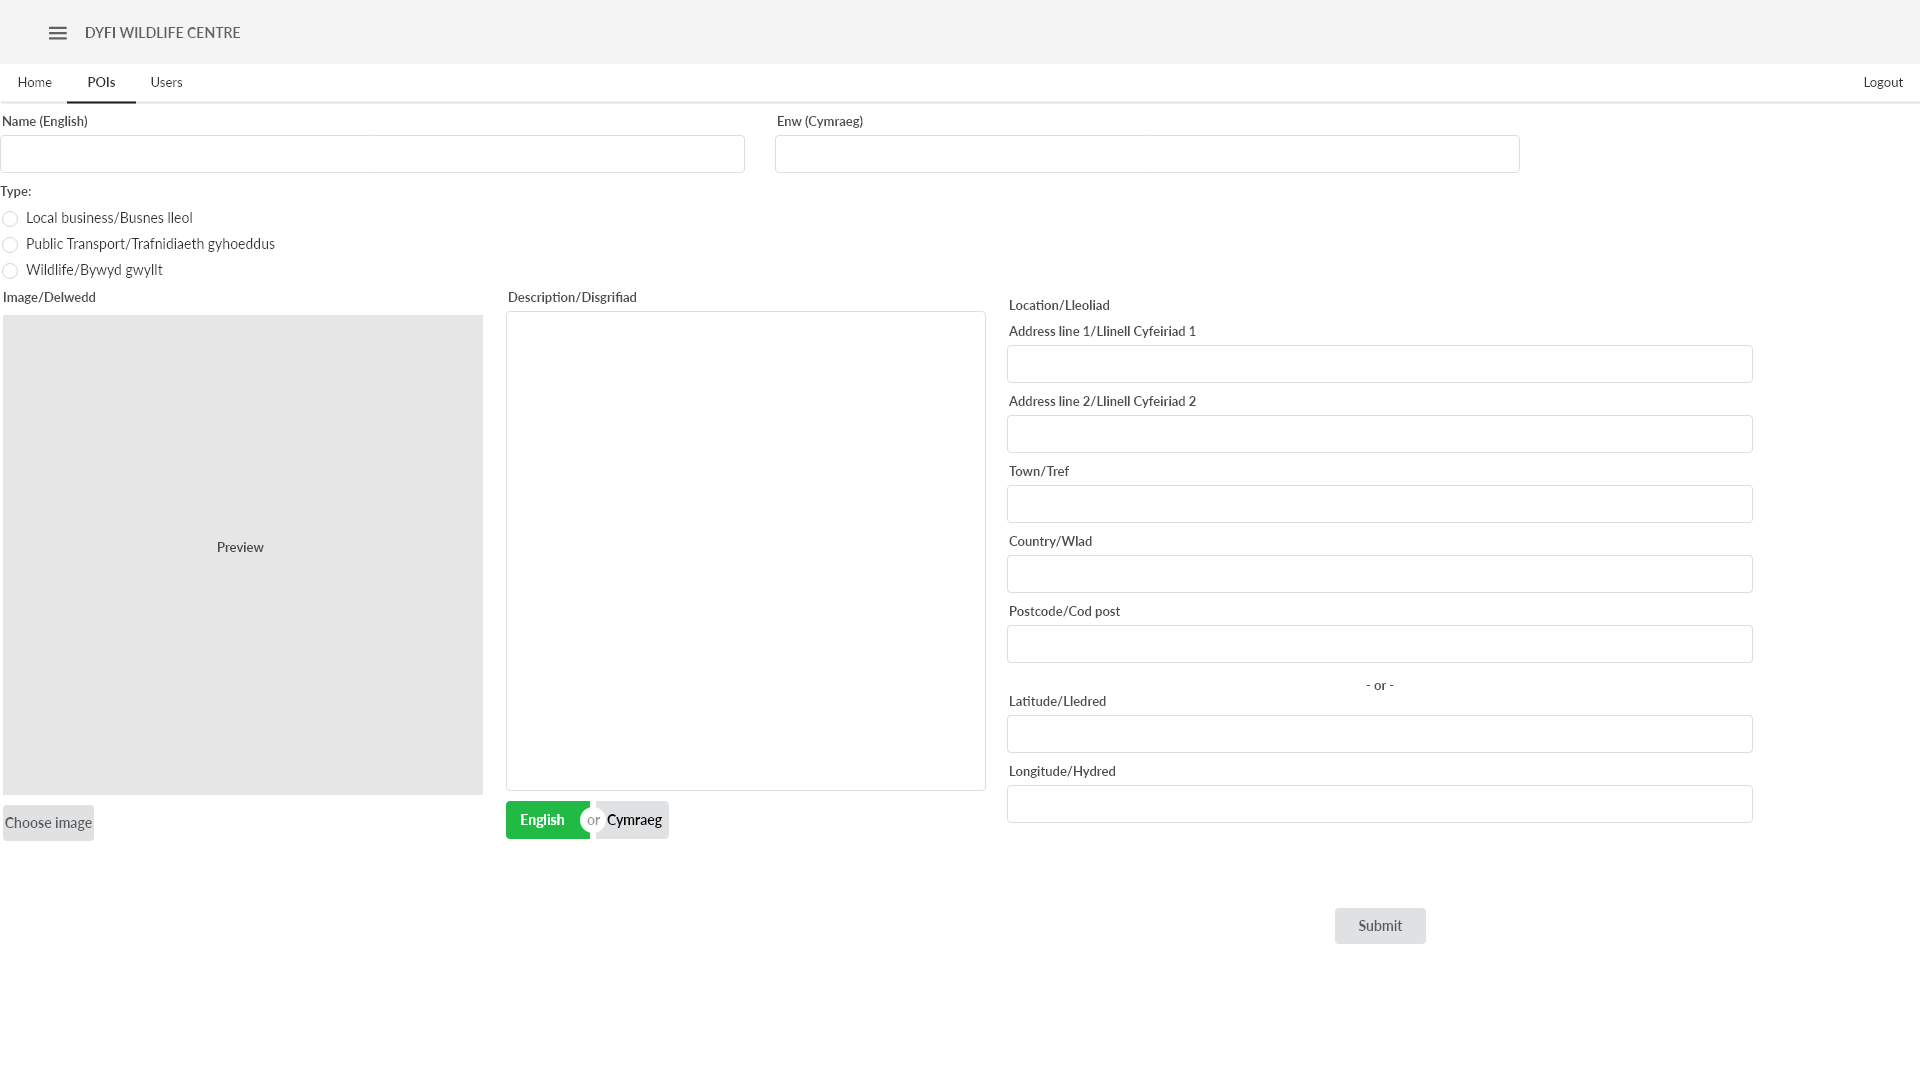
\includegraphics[scale=0.2]{mockups/Admin Panel - POIs (not filled, English)}
\caption{Mockup of the POI editing prompt}
\end{figure}

The initial logic behind the POI editing screen allowed for an entire address to be added, and a coordinate pair if it was deemed necessary by the user. Ultimately, this was considered an overcomplicated solution, and, as explained above, either a postcode or a coordinate pair were required.
\newpage
\subsubsection{Admin Panel - User management}
\begin{figure}[!htbp]
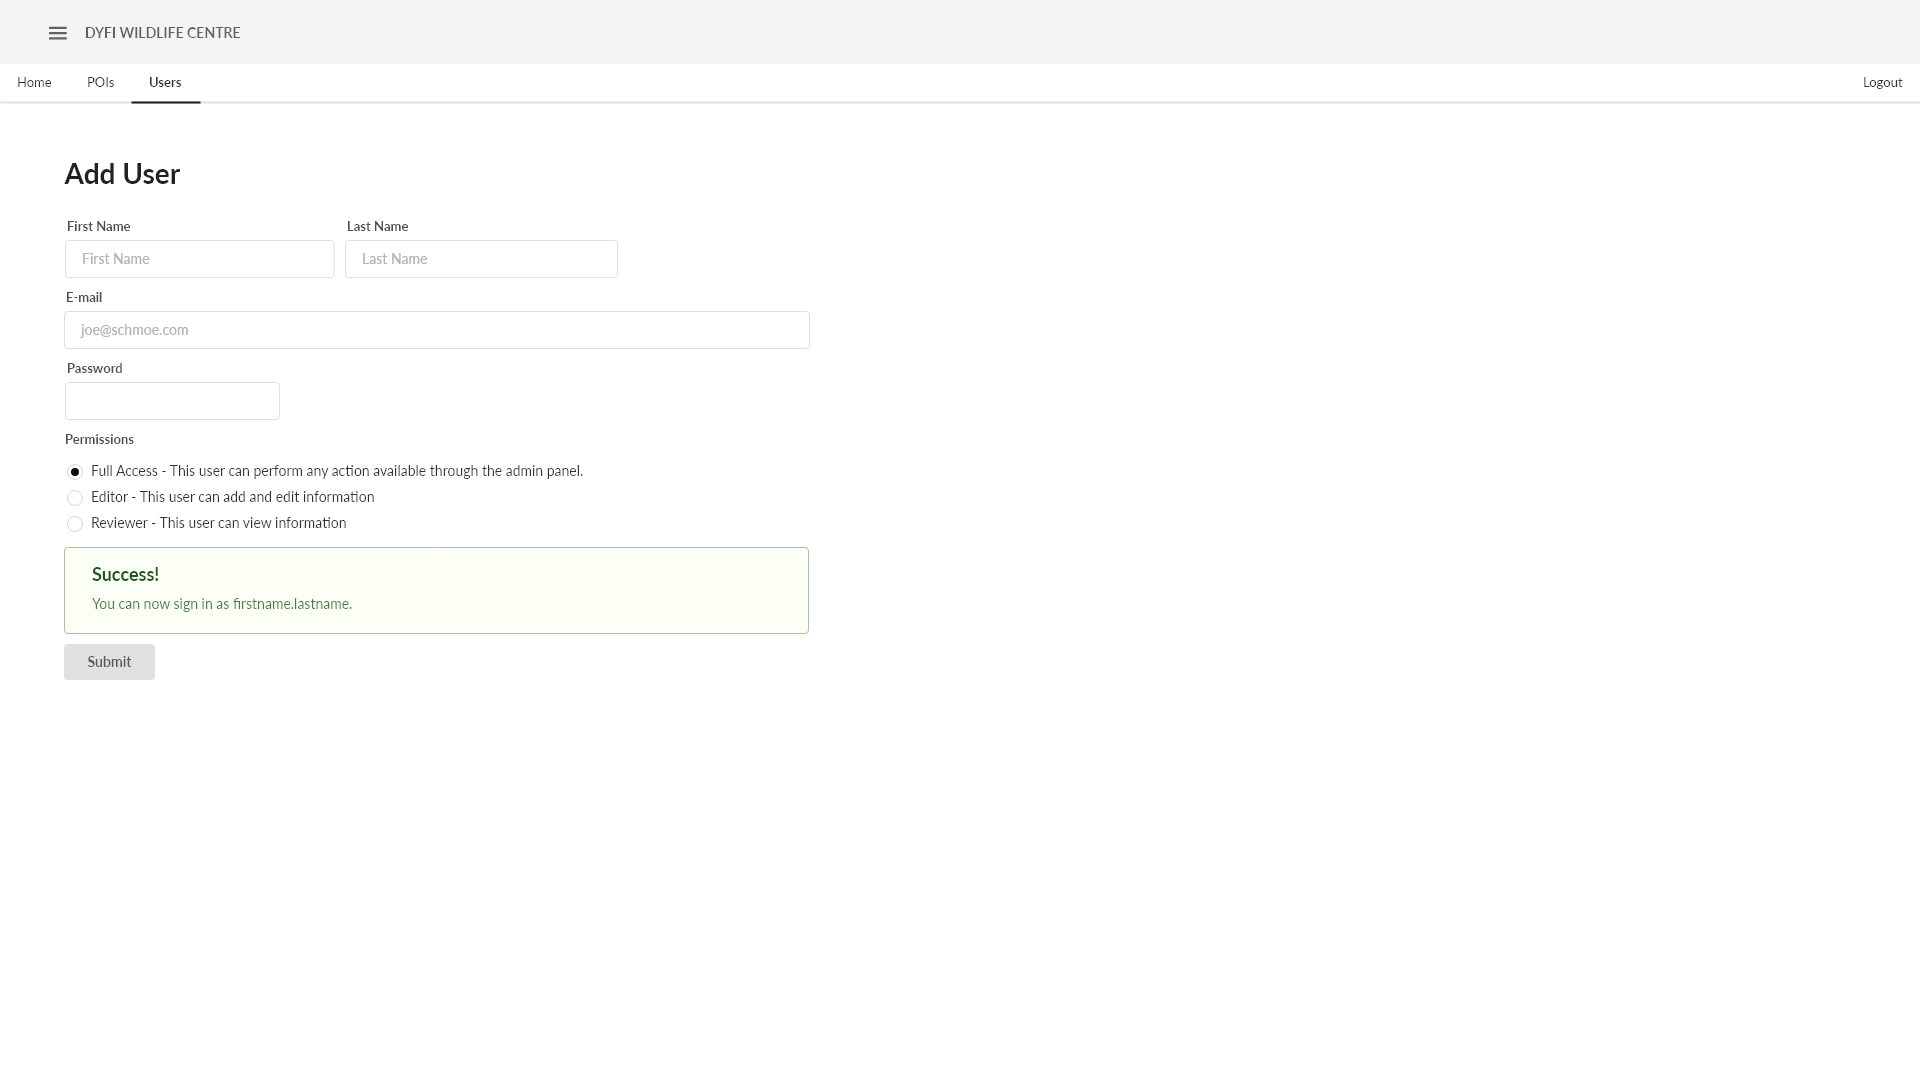
\includegraphics[scale=0.2]{mockups/Admin Panel - Add User}
\caption{Mockup of the 'Add a user' screen}
\end{figure}

Similarly, adding a user with various details was later decided as relatively redundant, as a simple username and password would suffice for security purposes. Changes in decisions made will be discussed in Chapter 3.

%Chapter 2: 3244 words
%Total: 6567 words